\documentclass[../main.tex]{subfiles}
\graphicspath{{\subfix{../images/}}}


\begin{document}

In this chapter we give technical details about the methods used to perform statistical postprocessing of rainfall forecasts. We begin by outlining the data that was used to train and validate on in Sec.~\ref{sec:data}, before discussing the particular machine learning model setup that we have used in Sec.~\ref{sec:model_setup}. We then outline the quantile mapping approach that we use to complement the cGAN approach and provide a strong baseline to compare against in Sec.~\ref{subsec:qm}, and the bootstrapping method used to assess sampling variability in Sec.~\ref{sec:sample_var}. 

\section{Data}
\label{sec:data}


For observational data, we use the Integrated Multi-satellite Retrievals for GPM (IMERG) V06B dataset; this is calculated through satellite observations of microwave and infrared by the array of Global Precipitation Measurement (GPM) satellites, with subsequent calibration incorporating rain gauges~\citep{huffman_nasa_2018}. The observations are half-hourly at a resolution of $0.1^{\circ} \times 0.1^{\circ}$ ($11\text{km} \times 11\text{km}$ at the equator), with precipitation rates given in mm/hr representing the average rainfall over the entire half hour period\footnote{\href{https://gpm.nasa.gov/data/imerg}{https://gpm.nasa.gov/data/imerg} accessed 29th November 2022}.


Whilst the IMERG data does not perfectly represent the true rainfall, it performs reasonably well at capturing the diurnal cycle and distribution of rainfall in East Africa~\citep{dezfuli_validation_2017, roca_comparing_2010, camberlin_major_2018} compared to other alternatives, particularly given the scarcity of reliable rain gauge and radar data in the area.  In~\cite{ageet_validation_2022} they compare a range of satellite rainfall estimating products including the IMERG product, by comparing the satellite estimates with rain gauges in an area around Uganda (including parts of Kenya, Tanzania, Sudan and the Democratic Republic of Congo) over 17 years. Based on a combined assessment of quantile-quantile plots, correlation, and skill scores such as hit rate and false alarms, they identify the IMERG product as the best performing at a daily level. However, it still has biases, for example it has a tendency to underestimate the rainfall rate, and over-predict the frequency of rainfall. There are also known issues with similar satellite products in mountainous areas~\citep{dinku_comparison_2010}, which means these observations may be more unreliable over areas such as the Ethiopian Highlands and parts of the Rift Valley. A dry bias has also been observed in several works (e.g.~\cite{vogel_skill_2018}). Overall though it provides a good source of large amounts of high temporal and spatial resolution data, and it has been used in other studies in this region (e.g.~\cite{woodhams_what_2018, finney_implications_2019, cafaro_convection-permitting_2021}).

% In~\citep{kimani_assessment_2017} they evaluate the predecessor to IMERG, the Tropical Rainfall Measuring Mission (TRMM) alongside other observations, and identify it as one of the best performing products in the area in terms of mean bias and correlation with rain gauges, although , 
% \hl{With the upcoming launch of the third generation Meteosat satellite, we expect ..https://www.eumetsat.int/meteosat-third-generation.}


The forecast used is the the ECMWF IFS HRES deterministic hourly forecast~\citep{ecmwf_operational_2023} (interpolated from $9\text{km} \times 9\text{km}$ resolution to $0.1^{\circ} \times 0.1^{\circ}$) as this tends to perform amongst the best compared to similar models~\citep{haiden_intercomparison_2012}. The model takes IFS forecast variables plus the orography and land-sea mask as inputs, and uses IMERG as the ground truth. Note that the land-sea mask labels lakes as well as sea, which is important given the presence of Lake Victoria and other nearby lakes. Since the IFS forecasts rainfall values are cumulative, we convert cumulative values to mm/hr values by finding the difference in cumulative values over the hour. So e.g.~for a forecast time of 1pm, the precipitation in mm/hr is the difference between the cumulative rainfall values at 1pm and 2pm. Instantaneous variables (like wind speed) are taken as the value on the hour, so e.g.~for a forecast time of 1pm, the wind speed is the value at 1pm. 




\section{Model setup}
\label{sec:model_setup}


Our model architecture uses the same architecture and code as in~\cite{harris_generative_2022}, itself based on~\cite{leinonen_stochastic_2020} in which a conditional Wasserstein GAN is trained to predict realistic rainfall patterns conditioned on several meteorological inputs together with constant inputs such as orography. Both the generator and discriminator are deep neural networks primarily made up of residual blocks that each contain two convolution layers, using square convolutional kernels of width 3 pixels. The generator is composed of 7 residual blocks (each with $f_g$ filters), with a final softplus activation function, giving a total of $2 \times 7 \times f_g$ hidden layers each of size $200 \times 200$. The discriminator is made up of 3 residual blocks (each with $f_d$ filters), and two dense layers, giving a total of $2 \times 3 \times f_d$ hidden layers each of size $200 \times 200$. 
Excluding the output layers, PReLU activation functions were used, were we set the $\alpha$ parameter for the PReLU to 0.2 following~\cite{harris_generative_2022}. The number of noise channels was set to 4, and the learning rates for the generator and discriminator were set equal to $1\times 10^{-5}$, with the discriminator being trained for 5 steps for every 1 step of generator training. In line with the settings in~\cite{gulrajani_improved_2017} we set the gradient penalty parameter $\gamma$ to 10. The batch size was set to 2 based on hardware memory constraints.

 On top of the 9 variables used in~\cite{harris_generative_2022}, we included 11 extra fields from temperature, convective precipitation, vertical velocity, and relative humidity (some of which are at several geopotential heights; see Appendix for a full table of inputs~\ref{app:fcst_vars}). Convective inhibition was included, with null values set to 0. IFS forecasts are provided at 00h and 12h and so for each observation the nearest forecast within a 6-18h window was selected, so that the lead time sits somewhere between nowcasting and short-range weather prediction (however it is expected that the method we use could also equally apply to longer lead times).

 In order to perform shorter experiments to tune hyperparameters, smaller models with $f_g=32, f_d=128$ were trained for $6.4\times 10^4$ iterations using the Adam optimiser, and then larger models with $f_g=64, f_d=256$ were trained for $3.2\times10^5$ steps; thus our largest model was smaller than the model in~\cite{harris_generative_2022} that had $f_g=128, f_d=512$, due to constraints on the hardware memory. The best model in the last 1/3rd of checkpoints was selected based on judgement of the combined performance on CRPS, RAPSD and mean squared error, plus visual evaluation of the samples produced. Our batch size was limited to 2 due to the need to generate an ensemble to calculate the loss function (discussed in the next paragraph). All models were trained on a single Nvidia A100 GPU.

One notable addition by Harris et.~al.~is the inclusion of a `content loss' term, inspired by~\cite{ravuri_skilful_2021}, which penalises GAN predictions that do not have an ensemble mean close to the observed value. Specifically, at each training step the generator produces an ensemble of predictions (set to 8 in this work), and the generator loss function is modified to include a mean-squared error term between the real image $\mathbf{y}_{\text{real}}$ and the ensemble mean of the generated samples:
\begin{align}
\label{eq:content_loss}
\tilde{\mathcal{L}}_G(\mathbf{y}_{\text{real}}, \mathbf{z}; \theta_G) = \mathcal{L}_G(\mathbf{z}; \theta_G) + \frac{\mathcal{\lambda}}{HW} \left\Vert \mathbf{y}_{\text{real}} - \frac{1}{N_E} \sum_{i=1}^{N_E} G(\mathbf{z}_i;\theta_G) \right\Vert_2^2
\end{align}
where $N_E$ is the size of the ensemble, $H$ the height of the image, $W$ the width of the image and $\lambda$ the content loss parameter. In~\cite{ravuri_skilful_2021} it was demonstrated that without the content loss term, the predictions tended to perform poorly on CRPS, CSI and power spectral density. Note there are significant differences in the content loss term used in~\cite{harris_generative_2022} to the implementation in~\cite{ravuri_skilful_2021}: Harris et. al. transform $\mathbf{y}_{\text{real}}$ according to $x \to \log_{10}(x+1)$, there is no clipped weighting term, and they used an $l_2$ in place of the $l_1$-norm used in~\cite{ravuri_skilful_2021}. 

During validation of the models, we observed that using log normalisation of the outputs, as done by Harris et.~al., produced a distribution of rainfall that tended to exponentially deviate from the observations at the extreme rainfall values, and so produced very unrealistic values of rainfall. To remedy this we experimented with removing the log normalisation for the output rainfall values, finding that this removed the unrealistic values, instead slightly under-predicting the rainfall. We chose to accept this trade-off since the non-log normalised version could be corrected by quantile mapping, and it is undesirable to have excessively unrealistic rainfall values. This also removed the need to apply a cutoff to the predicted rainfall value, as done in Harris et. al. This also required modifying the content loss parameter $\lambda$, with $\lambda=100$ appearing to produce the best results according to a joint assessment of CRPS, RALSD, and quantile-quantile plots.

The dataset was split up as follows:
\begin{itemize}
    \item Training set: March 2016 – February 2018 and July 2018 – Sept 2020 (excluding validation months)
    \item Validation set: Jun 2018, Oct 2018, Jan 2019, March 2019
    \item Test sets: October 2020 - September 2021, March - May 2018
\end{itemize}
The choice of the validation set is such that a month from each of the different seasons is used to gauge which model performs best over a range of typical scenarios. Note also that we leave out the 2018 long rains (March-May) to test against since this was a period of particularly heavy rainfall~\citep{kilavi_extreme_2018}, and so will shed light on how well the model extrapolates to extreme rainfall. 





     
\begin{figure}[h]
     \begin{subfigure}[c]{0.48\textwidth}
     \centering
         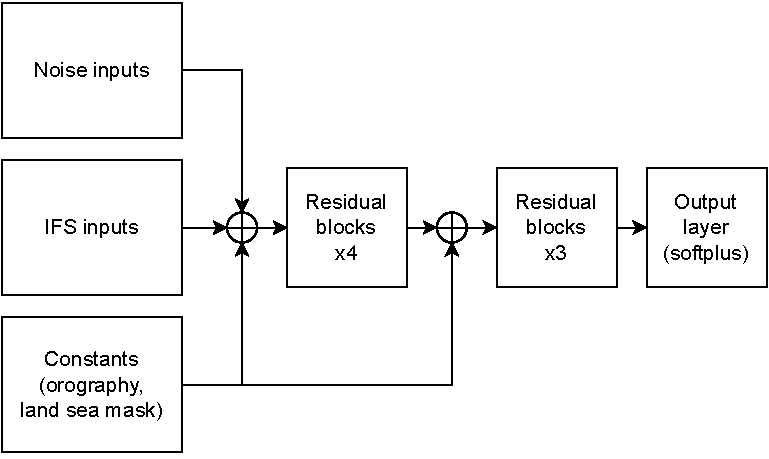
\includegraphics[width=\textwidth]{images/generator_2.drawio.pdf}
         \caption{}
         \centering
     \end{subfigure}
     \hfill
     \begin{subfigure}[c]{0.48\textwidth}
         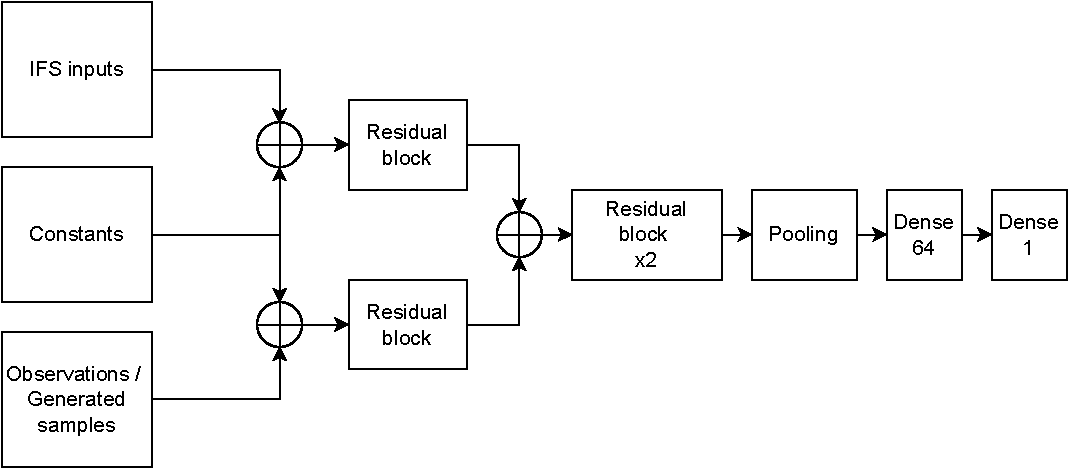
\includegraphics[width=\textwidth]{images/discriminator.drawio.pdf}
         \caption{}
         \centering
     \end{subfigure}
      \caption{The model architecture used in this work: a) the generator model and b) the discriminator model. For the generator, all inputs are first concatenated before being passed through 4 residual blocks. The output of this is concatenated with the constants again before being passed through another 3 residual blocks and a final output activation layer. The discriminator concatenates IFS inputs with constants, and constants with observations, which are then separately passed through residual block before being concatenated again, and passed through another 2 residual blocks. The outputs are then pooled and reshaped into a single number using two dense layers.}
     \label{fig:resnet}
\end{figure}    





% Using the smaller model we experimented with the two different types of content loss given in~\citep{harris_generative_2022} and \citep{ravuri_skilful_2021}, and were able to achieve better performance using the form in (\ref{eq:content_loss}) , perhaps because of training instabilities due to loss spikes caused by larger rainfall values. The value that achieved the best performance in terms of a balance of RALSD and CRPS was with $\lambda = 2000$.

In~\cite{harris_generative_2022} the training samples are chosen based on the total rainfall of each sample, such that wetter days are sampled more during training than drier days. However, the threshold used by Harris et. al.~for postprocessing UK rainfall was not appropriate for the drier region we are considering. We experimented with splitting data into rainfall by quartiles (according to mean rainfall over the image) and sampling the higher quartiles more often, but from visual inspection of the generated images this performed worse than just sampling uniformly over the training data, perhaps because we did not modify the loss function to compensate for the over-sampling.

Following standard practise for training neural networks, and based on the transformations applied in~\cite{harris_generative_2022}, we normalise the input variables: Precipitation input and variables are log normalised via $x \to \log_{10}(1 + x)$, whilst others were either divided by the maximum value, or normalised to fall within the maximum and minimum values (see Appendix~\ref{app:fcst_vars}).


Since our data volumes are relatively small compared to the amounts typically desired for deep learning, we used data augmentation to increase the variation of the samples the model sees, as this has been demonstrated to improve the generalisability of deep learning models~\citep{goodfellow_deep_2016}. To do so we randomly cropped the $270 \times 265$ images to smaller images of $200 \times 200$ during training. We also experimented with random rotations of multiples of $90^{\circ}$, however this led to a decrease in spatial realism (as measured by the quality of the RAPSD curve) and so was not used in the final run.



Similarly to the results in~\cite{harris_generative_2022}, we observed that the model quality during training (as measured by CRPS, RAPSD and visual inspection) was very variable, such that a validation set is required to pick the best model based on looking at summary statistics of CRPS, radially-averaged power spectral density, and ensemble mean-square error, plus visually assessing the realism of the samples. For this reason we kept out 4 months of validation data to be used to choose the best performing model (see Sec.~\ref{sec:data})



\section{Quantile mapping}
\label{subsec:qm}
Since it is known that raw IFS forecasts don't perform as well as post-processed forecasts in this region~\citep{vogel_skill_2018}, and IFS forecasts aren't intended to align with IMERG observations, we applied quantile mapping to the IFS forecasts (see e.g.~\cite{maraun_model_2017}) to provide a stronger baseline. Additionally, since our GAN predictions tended to over-predict at high rainfall values, we tested a variant of our model with quantile mapping applied to the output. In doing so we aimed to combine the strengths of both postprocessing methods to achieve an overall more accurate and realistic forecast. 
% A similar method to quantile mapping has been used within the African Monsoon Multidisciplinary Analysis 2050 (AMMA-2050) project, in which a model pipeline was built to produce reliable flood maps for future planning in Burkina Faso~\citep{senior_convection-permitting_2021}.


We used empirical quantile mapping rather than a distribution-based quantile mapping approach, since it has been demonstrated to work well~\citep{gudmundsson_quantile_2012}, and does not require a parametric distribution. Our method is based on the well-used methods outlined in~\cite{boe_statistical_2007, deque_frequency_2007, maraun_model_2017}, in which empirical cumulative density functions are calculated over the training period and used to create a mapping between the forecast quantiles and the observed quantiles. In general this means creating an estimate of the cumulative density functions $F_{f}$ and $F_{o}$ of the forecast and observations respectively, and mapping the forecast values $x_{f}$ to an adjusted value $\tilde{x}_f$ according to:
\begin{align}
    \tilde{x}_f = F^{-1}_o (F_f (x_f))
\end{align}

In~\cite{boe_statistical_2007}, percentiles at 1\% spacing are first calculated on the training set to find an approximation to the quantile distributions. Forecast values are then mapped into quantile values relative to the training data, and then converted into adjusted forecast values using the observed quantile values (using linear interpolation when the quantile falls between the known quantile values). 

Since the East African precipitation is low, there can be several quantiles that are 0; therefore if the forecast presents a 0 value there is no way to tell which quantile it belongs to. We follow the method in~\cite{boe_statistical_2007} and pick one of the 0-valued forecast quantiles at random, then assign the value of the matching observational quantiles. In practise, this can lead to low level noise on the corrected forecast, but replicates the high level statistics.

Based on the observation that evaluating the quantiles at high resolution was less important for lower quantiles, the step size between the quantiles was decreased towards the higher quantiles; so a step size of 0.01 was used up to 0.99, a step size of 0.001 used from 0.99 to 0.999, and so on until the step size cannot be reduced without having less than one data point per step (which is much higher resolution than seen in typical applications of quantile mapping, in order to capture the most extreme values). In practise this means going down to a minimum step size of $10^{-8}$, although note that each individual data point is far from independent and so the upper quantiles can be strongly affected by the presence of a single large weather system. This can lead to large errors due to the sampling variability in how the training and test sets are chosen, which we quantify using bootstrapping (see Sec.~\ref{sec:sample_var}).


% In previous works, high rainfall values have been dealt with in different ways; for example in~\citep{leinonen_stochastic_2020} all assessments were made after converting the rainfall values to the [0,1] range. 

For data greater than the maximum value observed in training, we follow the additive uplift method~\citep{boe_statistical_2007, deque_frequency_2007} and add the uplift of the highest quantile for the IMERG and IFS data. For example, if $o_{\text{max}},f_{\text{max}}$ are the highest values seen in the training set for the observations and forecast respectively, then for any forecast value in the test data greater than $f_{\text{max}}$ we add the uplift $(o_{\text{max}} - f_{\text{max}})$ to it. 

\begin{figure}[h]

    \centering
    \hspace{-20mm}
    \begin{subcaptionblock}{.4\textwidth}
        \centering
        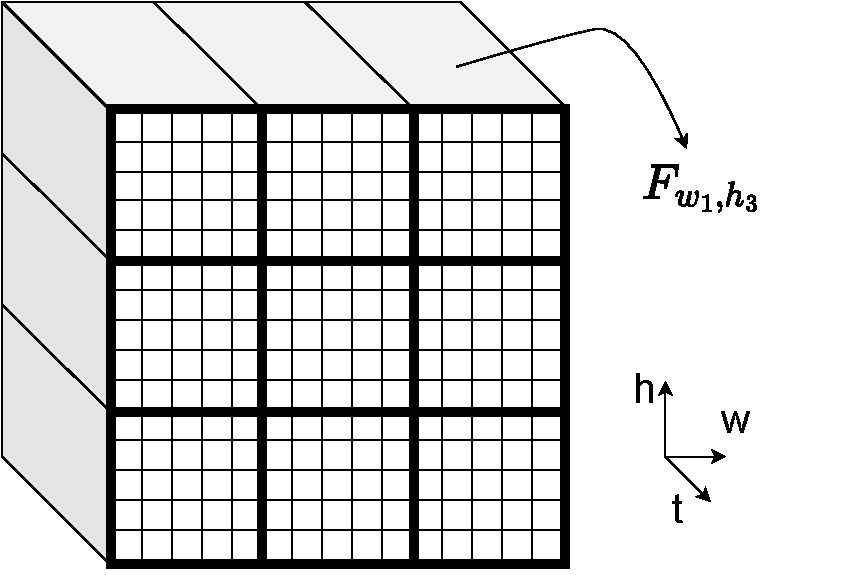
\includegraphics[width=\textwidth]{images/quantile_mapping.drawio.pdf}
        \caption{}\label{}
    \end{subcaptionblock}%
    \hspace{30mm}
    \begin{subcaptionblock}{0.20\textwidth}
        \centering
        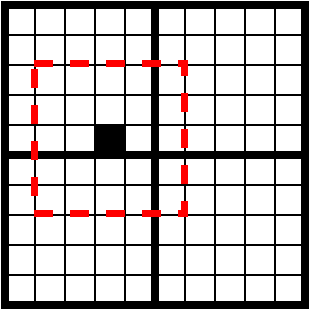
\includegraphics[width=\textwidth]{images/quantile_conv.drawio.pdf}
        \caption{}\label{}
    \end{subcaptionblock}%
    
        % \begin{subcaptionblock}{\label{cat}}
        % {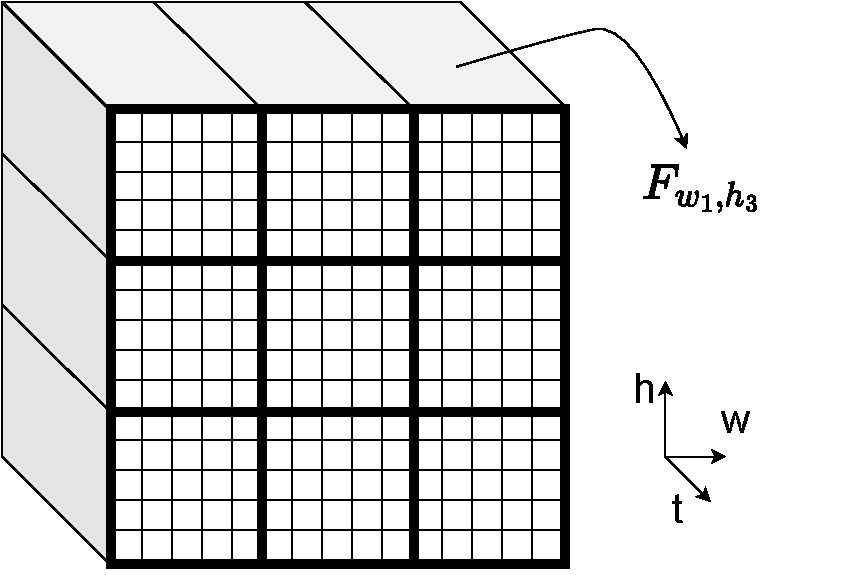
\includegraphics[width=0.5\textwidth]{images/quantile_mapping.drawio.pdf}}%
        % \subcaptionbox{\label{elephant}}
        % [0.5\textwidth]{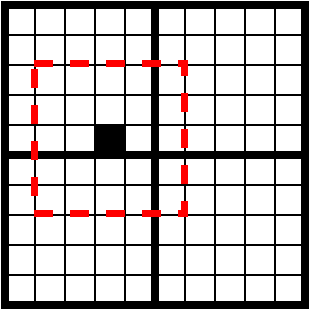
\includegraphics[width=0.25\textwidth]{images/quantile_conv.drawio.pdf}}
     % \begin{subfigure}[c]{0.48\textwidth}
     % \centering
     %     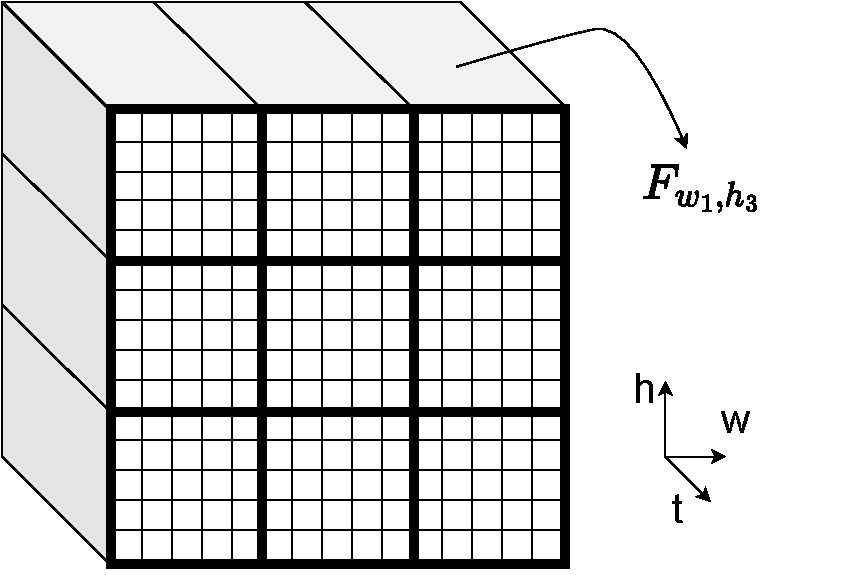
\includegraphics[width=\textwidth]{images/quantile_mapping.drawio.pdf}
     %     \caption{}
     %     \centering
     % \end{subfigure}
     % \hfill
     % \hspace{-10mm}
     % \begin{subfigure}[c]{0.25\textwidth}
     %     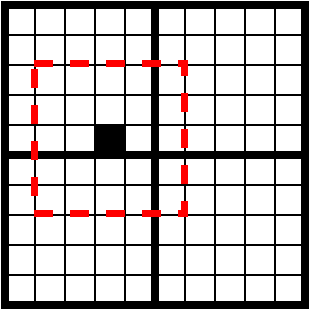
\includegraphics[width=\textwidth]{images/quantile_conv.drawio.pdf}
     %     \caption{}
     % \end{subfigure}
      \caption{a) Illustration of how grid cells are grouped together in order to estimate quantiles. In this example, the spatial domain is split into squares of $4 \times 4$ grid cells. Thus there are 9 separate square regions, and in each region the quantiles are calculated. b) to calculate a particular quantile for a grid point (in this case point (4,3)), we perform a weighted sum of the value of this quantile calculated in the square regions nearest to that pixel. The size of the weighting for each region is calculated by drawing a square around the grid cell (the red dashed line), and adding up how many small squares for each each region are contained in this square. In this example, the red dashed square covers 25 grid cells and the weightings would be $\frac{12}{25}$, $\frac{3}{25}$, $\frac{8}{25}$, $\frac{2}{25}$.}
     \label{fig:quantiles}
\end{figure}    


There are many other options possible for handling these values, such as fitting an extreme value distribution to the tails~\citep{kallache_nonstationary_2011, trentini_novel_2023}, or cutting values off at the largest value seen in training (effectively what is done in~\cite{leinonen_stochastic_2020} as all assessments were made after converting the rainfall values to the [0,1] range). The latter approach was deemed inappropriate for our use case in that it was too tied to the training distribution and didn't allow new extreme values to be predicted. The distributional approaches have the advantage of (perhaps) being reasonably well-behaved when dealing with data beyond the range of training data, with the downside of requiring an explicit parameterisation of the rainfall distribution. In our case, we observed that the tail distribution above 50mm/hr (extreme rainfall in this region is typically considered to be more than 50mm/hr over 6hrs~\citep{wilson_forecast_2014}) was not a straightforward fit to any common distributions, and instead tended to follow a power law up a certain point before falling exponentially (i.e.~a power law with exponential cutoff). Power laws are often observed due to mixtures of different behaviours~\citep{cavanaugh_probability_2015}, and the exponential cutoff could perhaps due to reaching a physical point beyond which it becomes prohibitive for increasing moisture to be stored in the atmosphere. So in order to fit a distribution to the tails, we would either have to model this physical limit (which is unlikely to be accurate) or fit another model to predict the point of exponential cutoff. For the sake of simplicity we therefore stick to the additive uplift method.

One further problem we encountered was the small number of independent training samples, which limited our ability to calculate accurate cumulative density. From experiments we found that the typical approach of quantile mapping the GAN at each grid point individually was not a robust approach for the extreme values. Therefore to calculate the quantiles we experimented with dividing the data into regions; spatially the region was grouped into equal sized squares (see Fig.~\ref{fig:quantiles} (a) for an illustration of this grouping). The intuition is that nearby points will have similar distributions and so we can gain accuracy by grouping nearby points together. 

To avoid any artefacts due to the edges of these domains, the quantiles for a given grid cell were calculated as a weighted average of the nearest squares; specifically, the quantiles used to update the values at grid cell $(m,n)$ are calculated as a weighted sum, where the weighting is calculated by drawing a square around $(m,n)$ and counting the number of grid points that fall into each quantile grouping (see Fig.~\ref{fig:quantiles} (b)). This is partly motivated by the ease of implementation, as this can be easily done by broadcasting the grouped quantiles to the same dimensions as the original grid, and using square convolutions with reflective padding to calculate the weighted versions of each quantiles. The length scale of the weighting window was chosen to be the same as the length scale of the quantile groupings, as this was empirically observed to produce reasonably smoothed values.

To evaluate the optimal grouping in the spatial domain, the mean square error of the quantiles after quantile mapping was evaluated over the whole domain. Using this method on the validation data, the cGAN performed best when quantiles were calculated uniformly over the whole domain, whilst the IFS forecast performed best when split into boxes of size $18 \times 18$. 


 
\section{Assessing sample variability}
\label{sec:sample_var}
Since our validation and training datasets are reasonably small, it is important to assess the effects of sampling variability by investigating the variance in the quantiles derived from the data; this gives insight as to where differences are due to model error and where they are due to sampling variability in the training and test sets. There are multiple approaches to do this; common approaches are via resampling methods such as subsampling and bootstrapping~\citep{efron_6_1982}. The subsampling approach involves estimating a quantity with $k$ samples removed from the data to infer the variance of the quantity. In the bootstrapping approach, many resampled datasets with the same dimension as the original are created by sampling with replacement from the full dataset, allowing an estimate of the variance in the quantity to be made. The two approaches approximate each other~\citep{efron_6_1982}, and in our case we observed negligible differences between the two, so we used bootstrapping. Another alternative is the Maritz-Jarrett method~\citep{wilcox_chapter_2022}, which calculates errors based on sums of the input variables weighted by incomplete Beta distribution functions; however, the standard Python implementation of this appeared to be much too slow for our data size.





% \begin{figure}[b]
%      \centering
%      \includegraphics[width=\textwidth]{Resnet_structure.png}
     
%      \caption{A schematic diagram of the generator network.}
%      \label{fig:resnet}
% \end{figure}
\ifSubfilesClassLoaded{%
    \bibliographystyle{alpha}
    \bibliography{references_z}

}{}


\end{document}